\documentclass[11pt]{article}
\usepackage{listings}
\usepackage{tikz}
\usepackage{enumerate}
\usetikzlibrary{arrows,automata,shapes}

\newtheorem{defn}{Definition}
\newtheorem{crit}{Criterion}

\newcommand{\handout}[5]{
  \noindent
  \begin{center}
  \framebox{
    \vbox{
      \hbox to 5.78in { {\bf Software Testing, Quality Assurance and Maintenance } \hfill #2 }
      \vspace{4mm}
      \hbox to 5.78in { {\Large \hfill #5  \hfill} }
      \vspace{2mm}
      \hbox to 5.78in { {\em #3 \hfill #4} }
    }
  }
  \end{center}
  \vspace*{4mm}
}

\newcommand{\lecture}[4]{\handout{#1}{#2}{#3}{#4}{Lecture #1}}
% 1-inch margins, from fullpage.sty by H.Partl, Version 2, Dec. 15, 1988.
\topmargin 0pt
\advance \topmargin by -\headheight
\advance \topmargin by -\headsep
\textheight 8.9in
\oddsidemargin 0pt
\evensidemargin \oddsidemargin
\marginparwidth 0.5in
\textwidth 6.5in

\parindent 0in
\parskip 1.5ex
%\renewcommand{\baselinestretch}{1.25}

% http://gurmeet.net/2008/09/20/latex-tips-n-tricks-for-conference-papers/
\newcommand{\squishlist}{
 \begin{list}{$\bullet$}
  { \setlength{\itemsep}{0pt}
     \setlength{\parsep}{3pt}
     \setlength{\topsep}{3pt}
     \setlength{\partopsep}{0pt}
     \setlength{\leftmargin}{1.5em}
     \setlength{\labelwidth}{1em}
     \setlength{\labelsep}{0.5em} } }
\newcommand{\squishlisttwo}{
 \begin{list}{$\bullet$}
  { \setlength{\itemsep}{0pt}
     \setlength{\parsep}{0pt}
    \setlength{\topsep}{0pt}
    \setlength{\partopsep}{0pt}
    \setlength{\leftmargin}{2em}
    \setlength{\labelwidth}{1.5em}
    \setlength{\labelsep}{0.5em} } }
\newcommand{\squishend}{
  \end{list}  }

\begin{document}

\lecture{7 --- January 19, 2015}{Winter 2015}{Patrick Lam}{version 2}

\section*{Further properties of paths} 
We've seen so far length-0 (NC), length-1 (EC) and length-2 (EPC) paths.
We could keep on going, but that gets us to Complete Path Coverage (CPC), which
requires an infinite number of test requirements.

\begin{crit}
{\bf Complete Path Coverage}. (CPC) \emph{TR} contains all paths in $G$.
\end{crit}

Note that CPC is impossible to achieve for graphs with loops.

Instead of going to CPC, we would like to capture ``the essence'' of
all loops. To do so, we first set up a few definitions:

\begin{defn}
A path is \emph{simple} if no node appears more than once in the path,
except that the first and last nodes may be the same.
\end{defn}

In the graphs above, {\sf some simple paths are:}\\[1em]
% $[n_1, n_2, n_3]$ or $[n_1, n_2, n_2]$
{\sf but not:}\\[1em]

Some properties of simple paths:
\squishlist
\item no internal loops;
\item can bound their length;
\item can create any path by composing simple paths; and
\item many simple paths exist (too many!)
\squishend
Because there are so many simple paths, let's instead consider
\emph{prime} paths, which are simple paths of maximal length.

\newpage
For instance, in the following graph:
\begin{center}
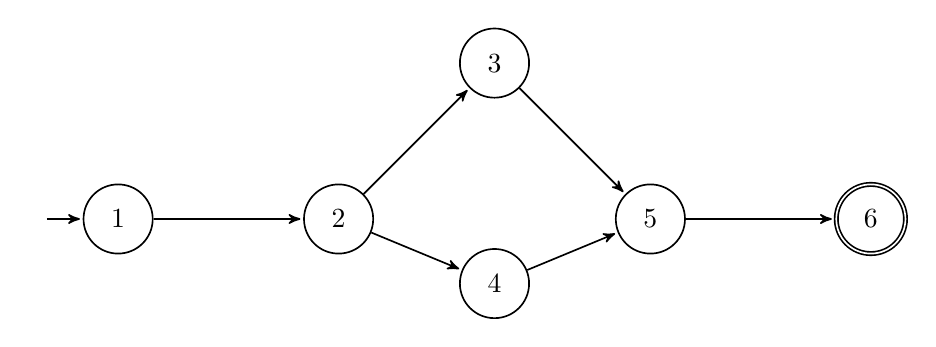
\begin{tikzpicture}[->,>=stealth',shorten >=1pt,auto,node distance=2.8cm,
                    semithick,initial text=]

  \node[initial,state]   (1)              {1};
  \node[state]           (2) [right of=1] {2};
  \node[state] (3) [above right of=2] {3};
  \node[state] (4) [below of=3] {4};
  \node[state] (5) [below right of=3] {5};
  \node[accepting,state] (6) [right of=5] {6};
  
  \path (1) edge              node {} (2)
        (2) edge              node {} (3)
        (2) edge              node {} (4)
        (3) edge              node {} (5)
        (4) edge              node {} (5)
        (5) edge              node {} (6);
\end{tikzpicture}
\end{center}
\begin{itemize}
\item {\sf Simple paths:}
\item {\sf Prime paths:}
\end{itemize}

\begin{defn} A path is \emph{prime} if it is simple and does not appear as
a proper subpath of any other simple path.
\end{defn}

\begin{crit}
{\bf Prime Path Coverage.} (PPC) \emph{TR} contains each prime path in $G$.
\end{crit}
There is a problem with using PPC as a coverage criterion: a prime path
may be infeasible but contain feasible simple paths.

{\sf Example:} \\[3em]
% double-diamond graph with first diamond (x > 5) and second diamond (x < 5).
% the prime path going through the two opposite branches is infeasible,
% but its subpaths are feasible.

One could replace infeasible prime paths in \emph{TR} with feasible subpaths,
but we won't bother.

\paragraph{Beyond CFGs.}
Let's now move beyond control-flow graphs and think about a different
type of graph. The next few graphs represent finite state machines
rather than control-flow graphs. Our motivation will be to set up
criteria that visit round trips in cyclic graphs.


\begin{center}
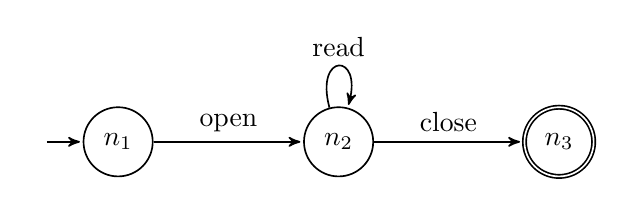
\begin{tikzpicture}[->,>=stealth',shorten >=1pt,auto,node distance=2.8cm,
                    semithick,initial text=]

  \node[initial,state]   (1)              {$n_1$};
  \node[state]           (2) [right of=1] {$n_2$};
  \node[accepting,state] (3) [right of=2] {$n_3$};
  
  \path (1) edge              node {open} (2)
        (2) edge              node {close} (3)
            edge [loop above]       node {read} (2);
\end{tikzpicture}
\end{center}
or perhaps
\begin{center}
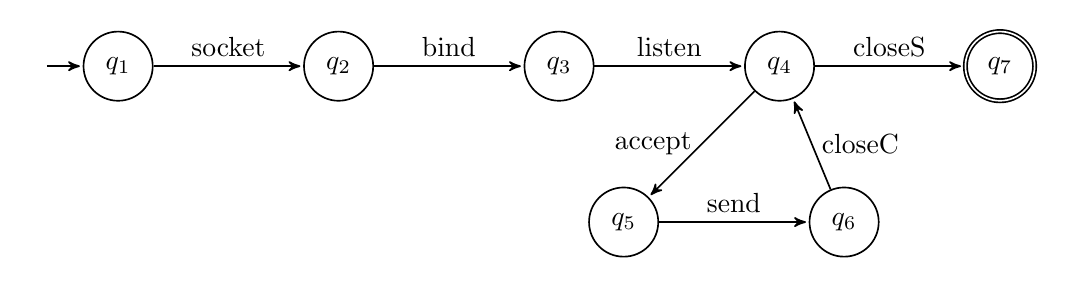
\begin{tikzpicture}[->,>=stealth',shorten >=1pt,auto,node distance=2.8cm,
                    semithick,initial text=]

  \node[initial,state]   (1)              {$q_1$};
  \node[state]           (2) [right of=1] {$q_2$};
  \node[state] (3) [right of=2] {$q_3$};
  \node[state] (4) [right of=3] {$q_4$};
  \node[state] (5) [below left of=4] {$q_5$};
  \node[state] (6) [right of=5] {$q_6$};
  \node[accepting,state] (7) [right of=4] {$q_7$};
  
  \path (1) edge              node {socket} (2)
        (2) edge              node {bind} (3)
        (3) edge              node {listen} (4)
        (4) edge              node {closeS} (7)
        (4) edge              node[left] {accept} (5)
        (5) edge              node {send} (6)
        (6) edge              node[right] {closeC} (4);
\end{tikzpicture}
\end{center}

Prime paths apply to both CFGs and other graphs. The next criteria
are mostly not for CFGs.
\begin{defn}
A \emph{round trip} path is a prime path of nonzero length that starts
and ends at the same node.
\end{defn}

\begin{crit}
{\bf Simple Round Trip Coverage}. (SRTC) \emph{TR} contains at least one
round-trip path for each reachable node in $G$ that begins and ends a
round-trip path.
\end{crit}

\begin{crit}
{\bf Complete Round Trip Coverage}. (CRTC) \emph{TR} contains all round-trip
paths for each reachable node in $G$.
\end{crit}

\paragraph{Exercise: Computing Prime Paths.}
Last time, we saw this graph:
\begin{center}
\begin{tikzpicture}[->,>=stealth',shorten >=1pt,auto,node distance=2.8cm,
                    semithick,initial text=]

  \node[initial,state]   (1)              {$1$};
  \node[state]           (2) [right of=1] {$2$};
  \node[state]           (3) [right of=2] {$3$};
  \node[state]           (4) [above of=3] {$4$};
  \node[state]           (5) [right of=3] {$5$};
  \node[state]           (6) [right of=5] {$6$};
  \node[accepting,state]           (7) [right of=6] {$7$};
  
  \path (1) edge              node {} (2)
        (2) edge              node {} (3)
            edge              node {} (4)
        (3) edge              node {} (5)
        (4) edge              node {} (5)
        (5) edge              node {} (6)
        (6) edge [bend left]  node {} (2)
        (6) edge              node {} (7);
\end{tikzpicture}
\end{center}
I recommend computing all of the simple paths for this example. (There are 53
simple paths, with length up to 5, and 12 prime paths.) Hint: write out
simple paths of length up to $N$. To get the simple paths of length $N+1$,
start with the paths of length $N$ and extend the ones that are extendable;
the non-extendable paths are prime, so mark them as you go along.

Here's another graph:
\begin{center}
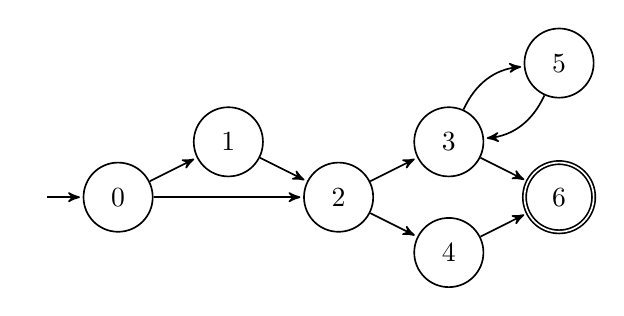
\begin{tikzpicture}[->,>=stealth',shorten >=1pt,auto,node distance=2.8cm,
                    semithick,initial text=]

  \node[initial,state]   (0)              {$0$};
  \node[state]           (1) [right of=0,xshift=-1.4cm,yshift=2em] {$1$};
  \node[state]           (2) [right of=0] {$2$};
  \node[state]           (3) [right of=2,xshift=-1.4cm,yshift=2em] {$3$};
  \node[state]           (4) [right of=2,xshift=-1.4cm,yshift=-2em] {$4$};
  \node[state]           (5) [right of=3,xshift=-1.4cm,yshift=1cm] {$5$};
  \node[accepting,state] (6) [right of=2] {$6$};
  
  \path (0) edge              node {} (1)
        (0) edge              node {} (2)
        (1) edge              node {} (2)
        (2) edge              node {} (3)
        (2) edge              node {} (4)
        (3) edge              node {} (6)
        (4) edge              node {} (6)
        (3) edge [bend left]  node {} (5)
        (5) edge [bend left]  node {} (3);
\end{tikzpicture}
\end{center}
This graph has 38 simple paths and 9 prime paths:
\[ [0, 1, 2, 3, 6], [0, 1, 2, 4, 6], [0, 2, 3, 6], [0, 2, 4, 6], [0, 1, 2, 3, 5], [0, 2, 3, 5], [5, 3, 6], [3, 5, 3], [5, 3, 5]. \]
To compute the prime paths, we could also enumerate all of the simple
paths and note non-extendable paths and cycles (which are both prime).
In doing so, one would also get all of the information necessary to
write out the test requirements for NC, EC and EPC. Since there is a
loop, it is impossible to explicitly write out all test requirements
for CPC, but one could write out some of them.

\end{document}
